\documentclass[11]{article}
\usepackage[margin=1in]{geometry}
\usepackage{amsfonts,amsmath,amssymb}
\usepackage{fancyhdr}
\usepackage{graphicx}
\usepackage{float}
\usepackage{transparent}
\usepackage{eso-pic}
\usepackage[colorlinks,linkcolor={blue}]{hyperref}



\usepackage{listings}
\usepackage{color}


\definecolor{dkgreen}{rgb}{0,0.6,0}
\definecolor{gray}{rgb}{0.5,0.5,0.5}
\definecolor{mauve}{rgb}{0.58,0,0.82}

\lstset{frame=tb,
  language=Java,
  aboveskip=3mm,
  belowskip=3mm,
  showstringspaces=false,
  columns=flexible,
  basicstyle={\small\ttfamily},
  numbers=none,
  numberstyle=\tiny\color{gray},
  keywordstyle=\color{blue},
  commentstyle=\color{dkgreen},
  stringstyle=\color{mauve},
  breaklines=true,
  breakatwhitespace=true,
  tabsize=3
}



\newcommand\BackgroundPic{%
\put(0,0){%
\parbox[b][\paperheight]{\paperwidth}{%
\vfill
\centering
{\transparent{0.3} 
\includegraphics[width=\paperwidth,height=\paperheight,%
keepaspectratio]{background.jpg}}%
\vfill
}}}

\AddToShipoutPicture*{\BackgroundPic}

\pagestyle{fancy}
\fancyhead{}
\fancyfoot{}
\fancyhead[L]{\slshape \MakeUppercase{Notes}}
\fancyfoot[C]{\thepage}
%\renewcommand{\headrulewidth}{0pt}
\renewcommand{\footrulewidth}{0pt}

\parindent 0ex
\renewcommand{\baselinestretch}{1.5}

\begin{document}
\begin{titlepage}
\begin{center}
\vspace{1cm}
\Large{\textbf{Computer Science 101: Introduction to Java and Algorithms}}\\
\vfill
\line(1,0){400}\\
\huge{\textbf{Section 4: Arrays}}\\
\line(1,0){400}\\
\vfill
Erudition Labs\\
Computer Science 101: Introduction to Java and Algorithms\\
\today\\
\end{center}
\end{titlepage}

\tableofcontents
\thispagestyle{empty}
\clearpage
\setcounter{page}{1}

\section{Terminology}
\begin{itemize}
  \item \textbf{\textit{Memory}} --
  Memory is where all the action happens. Many people often refer to it as storage space although that is not entirely true. When programmers talk of memory, we are talking about addressable memory. This means memory that computers can create addresses for and thus use. Memory is NOT hard drive space. It is RAM. The amount of memory you have depends on two things. The amount of RAM you have and the operating systems you are using (eg. 32 bit windows vs 64 bit windows). With 32 bit systems, you are limited to 4 GB of ram where as 64 bit machines are (theoretically since we haven`t done it) limited to 16.8 million terabytes of RAM. Everything happens in your memory. When you start up your computer, windows (or mac, linux, android, IOS...whatever) gets loaded into memory. Whenever you launch a program, it gets loaded into memory. Pretty much whenever you do anything on a computer, it`s done in memory. As a programmer, you generally deal with two types of memory, heap and stack. Refer to \autoref{sec:heap} to lean more about heap vs stack.

  
  \item \textbf{\textit{Data Structure}} -- Data structures is basically a term to describe a way of organizing data. We create certain rules for how we store and organize data so that we can take advantage of its organization when performing operations like insertion, retrieval, and searching. Some example data structures are arrays, linked lists, binary trees, hash maps and vectors. Feel free to look any up if you are curious. One of the simplest to understand is the linked list.
  
  \item \textbf{\textit{Collections}} -- In many programming languages we often come across the terms collections and containers. In Java, we only deal with collections. A collection is a way of grouping data together under the same name. I would recommend \url{<https://www.geeksforgeeks.org/collections-in-java-2/>} if you are curious about more.
  
  \item \textbf{\textit{Array}} -- A collection of data elements of the same type stored in a contiguous chunk of memory.
  
  \item \textbf{\textit{Elements of an array}} -- We use this phrase to talk about all of the pieces of data stored in an array.
  
  \item \textbf{\textit{Iterate over an array (loop over an array)}} -- We use these phrases when we are talking about using one of the loops, like a for or while loop, to look at each element in an array (one each iteration of the loop).
  
  \item \textbf{\textit{Random access}} -- This means we can access an arbitrary piece of memory. In reference to arrays, it means that we can access any arbitrary element in an array as long as it exists. You won`t hear this term too much until you learn about algorithm efficiency.
  
  \item \textbf{\textit{Index}} -- The position of something, often in an array-like collection. In reference to arrays, the index is the position that an element is stored at in the array.
  
  \item \textbf{\textit{Index into an array}} -- We are using the index (aka the position of an element in an array) to get the value of the element at that position in the array.
  
  \item \textbf{\textit{Allocate memory}} -- Whenever we need create variables, the compiler looks at the type of variable  (int, float etc) and sets aside the right amount of memory to store values of that type (aka allocate memory). However, in the case of things like arrays and object (more on objects later), the programmer need to allocate the memory. Basically, any time you use the ``new`` keyword, you are allocating memory for that type to store the values.
  
\end{itemize}
\section{Pre-Chapter}
\subsection{Heap and Stack Memory(Over Simplified)}
\label{sec:heap}
Programmers care about two types of memory which we refer to as ``the Stack`` and ``the Heap``. Really these will make more sense once you learn about data structures and learn what a stack and a heap is and how they work. However, when we say ``the`` before it, like ``the stack`` or ``the heap``, we are talking about two sections of memory. \\

Let us imagine that you have 8 GB or RAM. In reality your operating system and various other things will be using all that. Besides that, Java will limit how much memory you are allowed to have. But lets say, for instance, that Java allows us to have 2GB of memory. It`s just this huge chunk of addressable memory (meaning memory we can use). When we write a program, there are certain things that the compiler will already know. For example, you will define all of you variables. All of the stuff that the compiler can know before hand will be allocated to the stack memory. Now there are things that the compiler won`t be able to know before hand. For example, lets say that we want to create something once the program is already running (soon you will learn that we do this with arrays), all of this stuff gets allocated to the heap.\\

With the information that you have seen so far, all we can really say about the stack and the heap is that they really are all just one big chunk of memory, but we divide them up and make them follow rules. Most things that the compiler can know will go on the stack, while things we do dynamically when the program is running will go on the heap. Don`t worry, we will be revisiting these concepts quite a few times throughout the course, hopefully making the distinction clearer as we go.

\subsection{The ``new`` keyword}
This will probably be the first time that you see the ``new`` keyword, at least in this course. In short, this keyword is used for allocating things to the heap.
\subsection{Declaration vs. Initialization}
Declaring a variable is different from initializing a variable. For example, declaring a variable looks like this:
\begin{lstlisting}
int a;
\end{lstlisting}

We are telling the compile (aka declaring to the compiler) that we want it to set aside space to store an integer and we will be referencing that space as ``a``.  Notice that we do not assign anything to that variable. It is only declared to the compiler.\\

So if we look at this snippet, 

\begin{lstlisting}
int a = 5;
\end{lstlisting}

We  are assigning $5$ to the variable ``a``. This is what we call initialization. We first declare the variable and then initialize it to $5$. In this case we do the declaration and the initialization at the same time. 

However, we there is no reason why we cannot separate them.
\begin{lstlisting}
int a;
a = 5;
\end{lstlisting}

In this case the first line declares the variable, and the second line initializes the variable to $5$.\\

So declaration is used to tell the compiler to set aside memory and initialization puts that memory to use by giving the variable a value.

\section{Arrays (Video Series Lecture 20 and 21)}
This section introduces Arrays, which is a data structure that stores collections of elements. What is a data structure? Well a data structure is just a way organizing data by following certain rules when we store and retrieve it. By doing this, we can take advantage of the way the data is organized to make efficient algorithms. Some data structures are better at some things than others. It all depends on what you need to do. So when you take a data structures class (or look into it yourself) you will learn about different data structures (aka different ways of organizing data), their rules, their advantages, disadvantages and their best use cases.\\

For example, if your program is going to be doing a lot of retrieving, there are data structures that are great for that. If you need to do a lot of saving or insertions, we have great data structures for that too, but those might also not be the best for retrieving. There are often trade-offs when using them and it is up to the programmer to decide which ones are best for your task. For now, you don`t really need to know what a data structure is other than it`s a way if organizing data. If you are taking computer science classes, then there are entire classes dedicated to that topic. All you need to know right now is that an array is used to store a collection of things of the same type and are extremely good for random access (meaning I can get any arbitrary piece of data at any time efficiently as long as I know where it is at in the array).
\subsection{What does an Array Look Like?}
Arrays are contiguous chunks of memory. And they MUST be contiguous due to how we access the data. I will talk about that more later. Usually when we try to visualize and conceptualize what an array is, we draw it like this:\\

\begin{figure}[H]
	\centering
	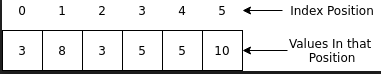
\includegraphics[scale=0.5]{arrays1.png}
	\caption{Image from Lecture}
\end{figure}

Imagine, if you will, having a bunch of variables of the same type under one name. This is essentially what an array is. So if you need to store a collection of integers, you can declare one array to store them instead of declaring a bunch of different variables. If you look at the table, the top row corresponds to the index position of the array. The index is simply where that particular piece of data is stored at in the array. Also note that we refer to these ``pieces of data`` as elements. For example, if we look at the table above, we can see that $8$ is an element of that array at index position $1$. \\

Notice that we start counting from $0$. The $0$th element is actually the first element in the array. Next, you can see all the boxes (aka the elements). Think of each box as a variable that you don`t have to name that stores a value. So in the image, we have an array of size $6$ that stores $6$ integers.\\

\subsection{Declaring/Initializing an Array}
We can declare an array just like we declare any other variable, in the form of
\begin{lstlisting}
int myArray[];
\end{lstlisting}
Now that we have declared the array, the compiler knows what we are talking about, but we cannot use it. Before we can use an array, we must initialize it with a size. We do that with the ``new`` keyword.

\begin{lstlisting}
int myArray[];
myArray = new int[10];
\end{lstlisting}
Java guarantees that the elements in the array allocated using new will automatically be initialized to zero (for numeric types), false (for boolean), or null (for when you learn about objects). Why does this matter? Because bad things happen when we try to access memory that has ``nothing`` in it. We will talk about it further in the ``Gotchas``  \autoref{sec:gotchas}. \\

Now lets briefly look at other common ways to declare and initialize arrays.

\begin{lstlisting}
int myArray[]; //declare
myArray = new int[10]; //initialize separately
//----------------------------------------

int myArray[] = new int[10] //initialize in one line
//----------------------------------------

int size = 5;
int myArray[] = new int[size]; //use variable for size
//----------------------------------------

int size = 5;
int myArray[]; //declare
myArray = new int[size]; //initialize separately

//-------------------------------------
int[] myArray = new int[] {5, 7, 3, 9, 10, 15, 27};
//create array and assign values to each position
\end{lstlisting}

\subsection{Accessing Elements}
To access elements, we need to know the position of the element in the array. The best way to see what I`m talking about is to let the code talk.

\begin{lstlisting}
class Main {
  public static void main(String[] args) {
    String myArray[] = new String[2]; //create array of size 2
    //access array using index
    myArray[0] = "hello"; // first element
    myArray[1] = "world"; // secodn element

    System.out.println(myArray[0] + " " + myArray[1]);
  }
}
\end{lstlisting}

At the beginning of the code, we create a String array of size two. So our array would look like this:
\begin{center}
	\begin{tabular}{ | c | c | } \hline
 	null & null  \\   \hline
	\end{tabular}
\end{center}

The next line, we access the first element of the array and set it equal to `` hello``. So now our array looks like this:

\begin{center}
	\begin{tabular}{ | c | c | } \hline
 	``hello`` & null  \\   \hline
	\end{tabular}
\end{center}

Then we do the next index position and set it to ``world``. 

\begin{center}
	\begin{tabular}{ | c | c | } \hline
 	``hello`` & ``world``  \\   \hline
	\end{tabular}
\end{center}

Finally we just print the the element at index $0$ concatenated with an empty space (so we have a space between out words so it looks like ``hello world`` instead of ``helloworld``) which is also concatenated with ``world``. So the output of this program is ``hello world``.	

\section{Looping Over Arrays (Video Series Lecture 22 and 23)}
Often times we need a way of looking at all of the elements in a given array (perhaps you are searching for an element for example or you would like to print out all of the elements). You can use the different types of loops to loop over the array. The most common loop used is the for loop since it maintains the current index with the current iteration. For example, If we want to search for an element in an array and print it out, we could do something like:

\begin{lstlisting}
class Main {
  public static void main(String[] args) {
    int[] myArray = new int[] {5, 7, 3, 9, 10, 15, 27}; //create array with values
    for(int i=0; i<myArray.length; i++) {
      if(myArray[i] == 9) {
        System.out.println("We found a 9 at array position " + i);
      }
    }
  }
}
\end{lstlisting}
In this code, we create an array and set values. We use the for loop to iterate until the variable $i$ reaches the number of elements (aka we loop to the end). Then we use variable $i$ to index into the array to get the value at that position and compare it to $9$. When the if statement evaluates to true, we execute the print statement. So the output of this code is ``We found a 9 at array position $3$``. If you look at the array we created, starting from $0$, you will see that there is a $9$ at position $3$ of the array.\\

Now let`s we want to print out all of the elements in the array? Can we simply do this:

\begin{lstlisting}
class Main {
  public static void main(String[] args) {
    int[] myArray = new int[] {5, 7, 3, 9, 10, 15, 27}; //create array with values
	System.out.println(myArray); // Can we do this? NOOOOOOO
  }
}
\end{lstlisting}

Turns out, we cannot do this. If you were to try, your output will look something like, ``[I@4aa298b7``. What the heck is that? Well to put it simply, you can think of that as the address in memory where the beginning of the array is stored.\\

So how do we print out all of the elements? Well you have to loop over each one and print it out.

\begin{lstlisting}
class Main {
  public static void main(String[] args) {
    int[] myArray = new int[] {5, 7, 3, 9, 10, 15, 27}; //create array with values
    for(int i=0; i<myArray.length; i++) {
      System.out.print(myArray[i] + " ");
    }
  }
}
\end{lstlisting}

This outputs ``0 1 2 3 4 5 6``

Or similarly with a while loop,
\begin{lstlisting}
class Main {
  public static void main(String[] args) {
    int[] myArray = new int[] {5, 7, 3, 9, 10, 15, 27}; //create array with values
    int i = 0;
	while(i < myArray.length) {
		System.out.print(myArray[i] + " ");
		i++;	
	}    
  }
}
\end{lstlisting}
\subsection{Increasing/Decreasing the size of an Array}
Can we take an existing array and increase or decrease it`s size? No. Sooooooo, now what? If you need to increase of decrease the size of an array, then you need to initialize a new array and use a loop to copy all of your elements over into the new array and assign your old array to your new array. Let`s let the code talk.

\begin{lstlisting}
class Main {
  public static void main(String[] args) {
    double myArray[] = new double[10]; //create array of size 10

    //OH NO, I ran out of room!!!

    double tempBiggerArray[] = new double[myArray.length * 2]; //new bigger temp array twice the size of my other array
    for(int i=0; i<myArray.length; i++) { //loop over old array of size 10
      tempBiggerArray[i] = myArray[i]; //copy over each element
    }
      myArray = tempBiggerArray; // now myArray has size 20
  }
}
\end{lstlisting}

As you can imagine, this seems like it isn`t an efficient thing to do every time you need more space (I say seems like because this if you are familiar with how a vector works, this is exactly what it does and it turns out that doubling the size of the array each time usually means that it only has to do so a handful of times.). This is a limitation of arrays. They must be initialized with a fixed length. And the size must be known at the time of initialization. This means that I must know how big I need my array to be so that I can create one big enough. And if I need one bigger, then I must create an entirely new array.

\section{2D Arrays (Video Series Lecture 24 and 25)}
Imagine having the need to represent a 2 dimensional matrix to perform linear transformations on in a game. Or even a 3 dimensional matrix for 3d game transformations or translations. What if I need a collection where each collection stores more collections? Well, it turns out that you can have nested arrays. Arrays of Arrays of Arrays and Nth dimensional arrays. Usually, however, we never really need to go beyond two or three dimensions, especially since each dimension will most likely add a performance penalty in your code.\\

All of the concepts are pretty much the same. We create them in the same way and index into them in a similar way. The only difference is that we need two indices now. Let`s take a look at this snippet of code where we create a $3$ x $3$ matrix and print it out:

\begin{lstlisting}
class Main {
  public static void main(String[] args) {
    int[][] myArray = new int[3][3]; //create 3x3 array filled with 0

    for(int i=0; i<myArray.length; i++) { //for each row
      for(int j=0; j<myArray[i].length; j++) { //for each column
        System.out.print(myArray[i][j]);
      }
      System.out.println(); //new line for each row
    } 
  }
}
\end{lstlisting}

The out put will look like this\\
0 0 0\\0 0 0\\ 0 0 0\\

When we create a new 2d array, it is often useful to thing of it as row by column, so ``new int [row][col]``, which in this case was just 3 x 3. Notice here that we used two for loops. When visualizing this, I think it is best to think of a 2d array simply as a 1d array that points to another 1d array.

\begin{figure}[H]
	\centering
	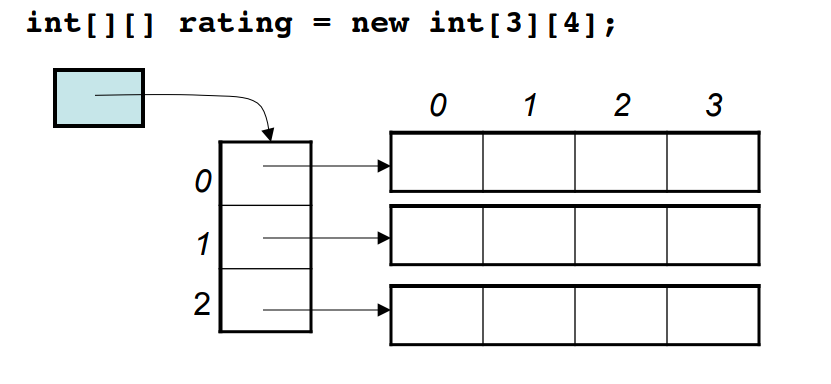
\includegraphics[scale=0.4]{2darray.png}
	\caption{Image from \url{<https://www.cs.cmu.edu/~mrmiller/15-110/Handouts/arrays2D.pdf>}}
\end{figure}

The first for-loop selects which row we want to iterate over. So the the first for-loop condition compares the counter $i$ to the number of rows in the 2d array. The second for-loop iterates over all of the elements in that row (aka the columns). This is why we use the length of the current row in the second for-loop condition. In other words, we are using the second for-loop to iterate over the $i-th$ row in the the 2d array.

\subsection{Another Example}
In this example we are going to create a a 2d matrix of strings. Each element will be the $x$ and $y$ coordinate of that 2d grid. Then we will print out the matrix.

\begin{lstlisting}
class Main {
  public static void main(String[] args){
    String[][] myArray = new String[4][6]; //create 4x6 array filled with 0

    for(int i=0; i<myArray.length; i++) {
      for(int j=0; j<myArray[i].length; j++) {
        myArray[i][j] = new String("(" + i + ", " + j + ")");
      }
    }

    for(int i=0; i<myArray.length; i++) { //for each row
      for(int j=0; j<myArray[i].length; j++) { //for each column
        System.out.print(myArray[i][j]);
      }
      System.out.println(); //new line for each row
    } 
  }
}
\end{lstlisting}

The output of this program will look like:\\
(0, 0)(0, 1)(0, 2)(0, 3)(0, 4)(0, 5)\\(1, 0)(1, 1)(1, 2)(1, 3)(1, 4)(1, 5)\\(2, 0)(2, 1)(2, 2)(2, 3)(2, 4)(2, 5)\\(3, 0)(3, 1)(3, 2)(3, 3)(3, 4)(3, 5)\\

We will be getting more practice with 2d arrays when we do our project at the end of the next chapter. We will be using a 2d array to represent out 2d world.

\section{Sorting Arrays: Insertion Sort Algorithm (Video Series Lecture 26 and 27)}
\section{Gotchas with Arrays}
\label{sec:gotchas}
\subsection{Array Index Out of Bounds}
The number one problem that you will face, I still face and what every programmer to ever exist has faced is the infamous ``ArrayIndexOutofBoundsException``. At least that`s what it is called in Java. If you ever compile your program and get this error, or you program crashes and you get this error, then go find where you are looping over arrays, because the problem is probably there. This exception means that you are overstepping the bound of your array. What does that mean? That means that you are using in index that is either bigger or smaller than the size of your array.\\

For instance, lets say that you created a 3 x 3 array. If you try to access this array with, say, [4][3], you will get that error because the the number of rows that your array has is 3 but you are trying to access the 4th element in the 5th row, which obviously doesn`t exist since you didn`t create it. Similarly with 1d arrays, if you create an array of size 6 then try to access the 10th element, you will get this error because it doesn`t exist.\\

This commonly happens when you are looping over your array. Sometimes you get into an infinite loop and the counter is greater than the size of your array. Many times, your loop condition is wrong and you will be off by one. Another common occurrence is when you are looping over the array backwards. Sometimes you still go too far and your counter becomes negative. If obviously doesn`t make sense to be accessing the element at position $-1$ of your array.\\

So if you come across this error, double check your loops, your loop conditions, your indices that you are trying to use and make sure you are using the right size arrays.

\section{Arrays Behind the Scenes}
Please note that you can totally skip this section if you like and it will definitely be helpful to go back to the first chapter and review of we deal with sizes of integers and units we use. However, if you are like me, you are probably asking why. Why must arrays be contiguous? Why must we allocate entirely new arrays when we want to increase of decrease the array size? Why must we know how many elements we are going to need to store? Why do we get an error when our index is greater or smaller than the size of the array? Well, I`m going to break down how arrays work.\\

If you look at lower level languages, especially C, you can get a clearer idea of what is going on. In C we deal with memory addresses directly. Java doesn`t give you a choice, you aren`t allowed to deal with them directly. So one way to create an array in C is as like this:

\begin{lstlisting}
int *A = (int *) malloc( 10 * sizeof(int));
\end{lstlisting}

Now there is no need for you to know what all of this means exactly. The variable $A$ is a pointer, which just means that it stores the memory address of where the variable is stored. the ``(int *)`` is called a cast. Malloc is a C function (we will talk about methods and functions in the next chapter) that returns a void pointer. So the ``(int *)`` tells the computer that we want to make that void pointer into an integer pointer. Next we have ``$10$ $*$ sizeof(int)``. There we are saying that we want  enough memory to store $10$ elements of the size of integers (often 4 bytes but depends on your system). So what does this give us exactly? It gives us the memory address of the first element of the array, and that`s it. So if all we have is the address of the first element of the array, how the heck are we supposed to do anything with it, and what is this indexing nonsense that we see in Java?\\

The array subscripts ``$[ ]$`` is sort of a shorthand notation or abstraction for what actually happens. To get the address of the $i-th$ element we need the base address and the data size. Since malloc gave us the base address and we know the data type, we have everything we need. The formula for getting the address of the $i-th$ element is $address$ $=$ $baseAddress$ $+$  $subscript$ $*$ $size$. The shorthand notation calculates exactly this and uses the address to get the value from memory.\\

Lets say we allocate a 1d array of 3 integer elements, where the size of the integers used on the system is 4 bytes and it just so happens that the base address ends up being $5000$.


\begin{figure}[H]
	\centering
	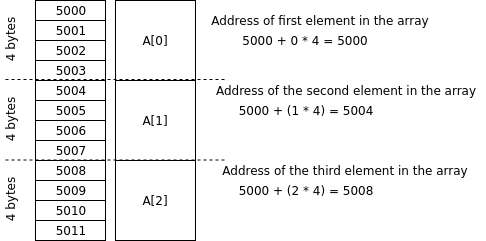
\includegraphics[scale=0.75]{rawarrays.png}
	\caption{Visual Representation}
\end{figure}

On the left is raw memory. On the right is the array elements. When dealing with memory, we generally deal with things in terms of bytes. So when each integer needs 4 bytes to represent the number, we take up 4 of the address spaces. The first element takes the address space of 5000 to 5003, the second 5004 to 5007 and the third 5008 to 5011. Next to each element, we use the subscript in the formula to calculate the address where each element is stored at in memory.\\

This is great and all, but what does all this have to do with the questions that we asked at the beginning? Well lets go through them. Why must arrays be contiguous? We now know that use the $[ ]$ to index into an array is the equivalent of using the formula to get the address where the element is stored. That is to say that indexing into an array is simply a math equation. What happens if it isn`t contiguous? What happens if there is a gap between the elements memory? If you look at the picture, what if there was a blank spot at address $5004$ and then the next array element starts. Well the rest of the calculations will be off by $1$ and when you go to index into the array, you are starting in the middle of the binary number. We are chopping off 4 bits of the rest of the numbers when we try to access them. On top of that, when we try to access the second element, there is nothing there, or there is random garbage there. Thus, arrays entirely rely on the fact that the memory is allocated contiguously.\\

Why must we allocate entirely new arrays when we want to alter the size of the array? If you read the pre-chapter, then you know that we allocate arrays using the ``new`` keyword, which means it gets allocated to the heap. Things that are allocated to the heap are done so sort of randomly. Since we usually never know what the size of something will be, it just finds a spot in memory in it. We have no guarantees that there will be any order to the heap. When we allocated our array in the image, it is entirely possible that there is something else stored at the address 5012. If we try to increase the array, then we would overwrite that value. Therefore, you must create an entirely new array since that is the only time that you are guaranteed that the memory will be allocated contiguously.\\

Why must we know how many elements we want to store? Well that`s easy to answer now. We need to know so we can allocate the right amount of memory.\\

Why do we an error when overstep the bounds of our array? As mentioned before, all we know is the address of the first element in the array. So what happens when we overstep the bounds? Well we try to access memory that wasn`t allocated for us. There is either nothing there, or some random garbage value. In other languages, such as C, there is nothing stopping you from overstepping the bounds. You simply access the garbage value, or in the case of nothing being there, the program just crashes. This was such a huge security problem that Java decided to do something about it. Java arrays actually know their size. They keep track of the array size so that when you try to overstep the bounds, it throws an error.
\end{document}